\section{\BENCHMARK{}}

\subsection{Problem Formulation}

The evaluation of \BENCHMARK{} requires an instance of 4-tuple $(\mathbf{S}, q, t_q, a)$. $\mathbf{S} \equiv [(t_1, S_1), (t_2, S_2), ..., (t_N, S_N)]$ is a sequence of $N$ history chat sessions ordered from the earliest to the latest, where $S_i$ is a multi-turn interaction between the user and a chat assistant and $t_i$ is the session's timestamp. {Each session can be further decomposed into rounds: one user message followed by one assistant response.} During test time, $\mathbf{S}$ is provided to the system one by one. $q$ and $t_q > t_N$ represent the question from the user and its date. $a$ is a short phrase indicating the answer, or a natural language rubric describing the preferred answer in the case where $q$ is open-ended.  

\subsection{{\BENCHMARK: Benchmark Curation}}
\label{section-benchmark-creation}

% \paragraph{Core Ability} 
One major challenge in building a reliable personalized assistant is performing online recording, recalling, updating, and reasoning on the dynamically evolving user information. To comprehensively reflect the challenge, \BENCHMARK{} formulates five core long-term memory abilities:

\begin{itemize}
    \item \textbf{Information Extraction (IE):} Ability to recall specific information from extensive interactive histories, including the details mentioned by either the user or the assistant. 
    \item \textbf{Multi-Session Reasoning (MR):} Ability to synthesize the information across multiple history sessions to answer complex questions that involve aggregation and comparison. 
    \item \textbf{Knowledge Updates (KU):} Ability to recognize the changes in the user's personal information and update the knowledge of the user dynamically over time.  
    \item \textbf{Temporal Reasoning (TR):} Awareness of the temporal aspects of user information, including both explicit time mentions and timestamp metadata in the interactions. 
    \item \textbf{Abstention (ABS):} Ability to identify questions seeking unknown information, i.e., information not mentioned by the user in the interaction history, and answer ``I don't know''. 
\end{itemize}

As shown in \Cref{tab:benchmark-comparison}, this formulation represents a more comprehensive ability coverage compared to prior long-term memory benchmarks like MemoryBank and PerLTQA. To thoroughly assess these abilities, \BENCHMARK{} features seven question types. \textbf{Single-session-user} and \textbf{single-session-assistant} test memorizing the information mentioned by user or assistant within a single session. \textbf{Single-session-preference} tests whether the model can utilize the user information to generate a personalized response. \textbf{multi-session} (MR) tests aggregating user information across two or more sessions. \textbf{knowledge-update} (KU) focuses on the ability to recognize changes in the user's life states and update the memory accordingly. \textbf{temporal-reasoning} (TR) tests reasoning with both the timestamp in metadata and explicit time references. Finally, we draw 30 questions from the previous question types and modify them into ``false premise'' questions, testing whether the model can correctly \textbf{abstain} from answering (ABS). \Cref{fig:main-fig-benchmark-examples} presents an example for each question type.

\paragraph{{Question Curation}} \Cref{fig:main-fig-benchmark-creation} depicts the question curation pipeline. We define an ontology of 164 user attributes in five categories: lifestyle, belongings, life events, situations context, and demographic information. For each attribute, we leverage an LLM\footnote{Unless otherwise mentioned, Llama 3 70B Instruct \citep{dubey2024llama} is used as the LLM in the pipeline.} to generate attribute-focused user background paragraphs, each of which includes detailed discussion of the user's life experience. To create a question, we randomly sample a paragraph and use an LLM to propose several seed (question, answer) pairs. As these LLM-proposed questions often lack depth and diversity, human experts manually filter and rewrite all the questions to achieve the desired difficulty. Then, we manually decompose the answer into one or more \textit{evidence statements} with optional timestamps. 

\paragraph{{Evidence Session Construction}} Each evidence statement is then separately embedded into a task-oriented \textit{evidence session} created by self-chatting \citep{xu-etal-2023-baize}. The user LLM is instructed to convey the evidence statement indirectly, e.g., instead of stating ``I bought a new car last month,'' it might instead ask for help about car insurance and reveal the information incidentally. This approach enhances the benchmark’s difficulty by requiring systems to recognize and memorize user details not explicitly emphasized in conversations. We present the full details in \Cref{appendix-dataset-construction}.

To ensure the data quality, all the evidence sessions are then manually screened and edited to (1) verify evidence inclusion, (2) distribute the evidence statement across different conversation positions, and (3) rephrase statements into more natural, colloquial language, especially for time mentions, which LLMs often express too formally. We also meticulously annotate the position of the evidence statement within each evidence session. For questions involving temporal information, we then manually add timestamps to both the evidence sessions and the questions. Most questions require evidence from multiple sessions (up to six) with evidence statements positioned diversely within sessions. \Cref{appendix-basic-statistics} presents further statistics of the final constructed data. 

\begin{figure}[t]
 \centering
\vspace{-3mm}
 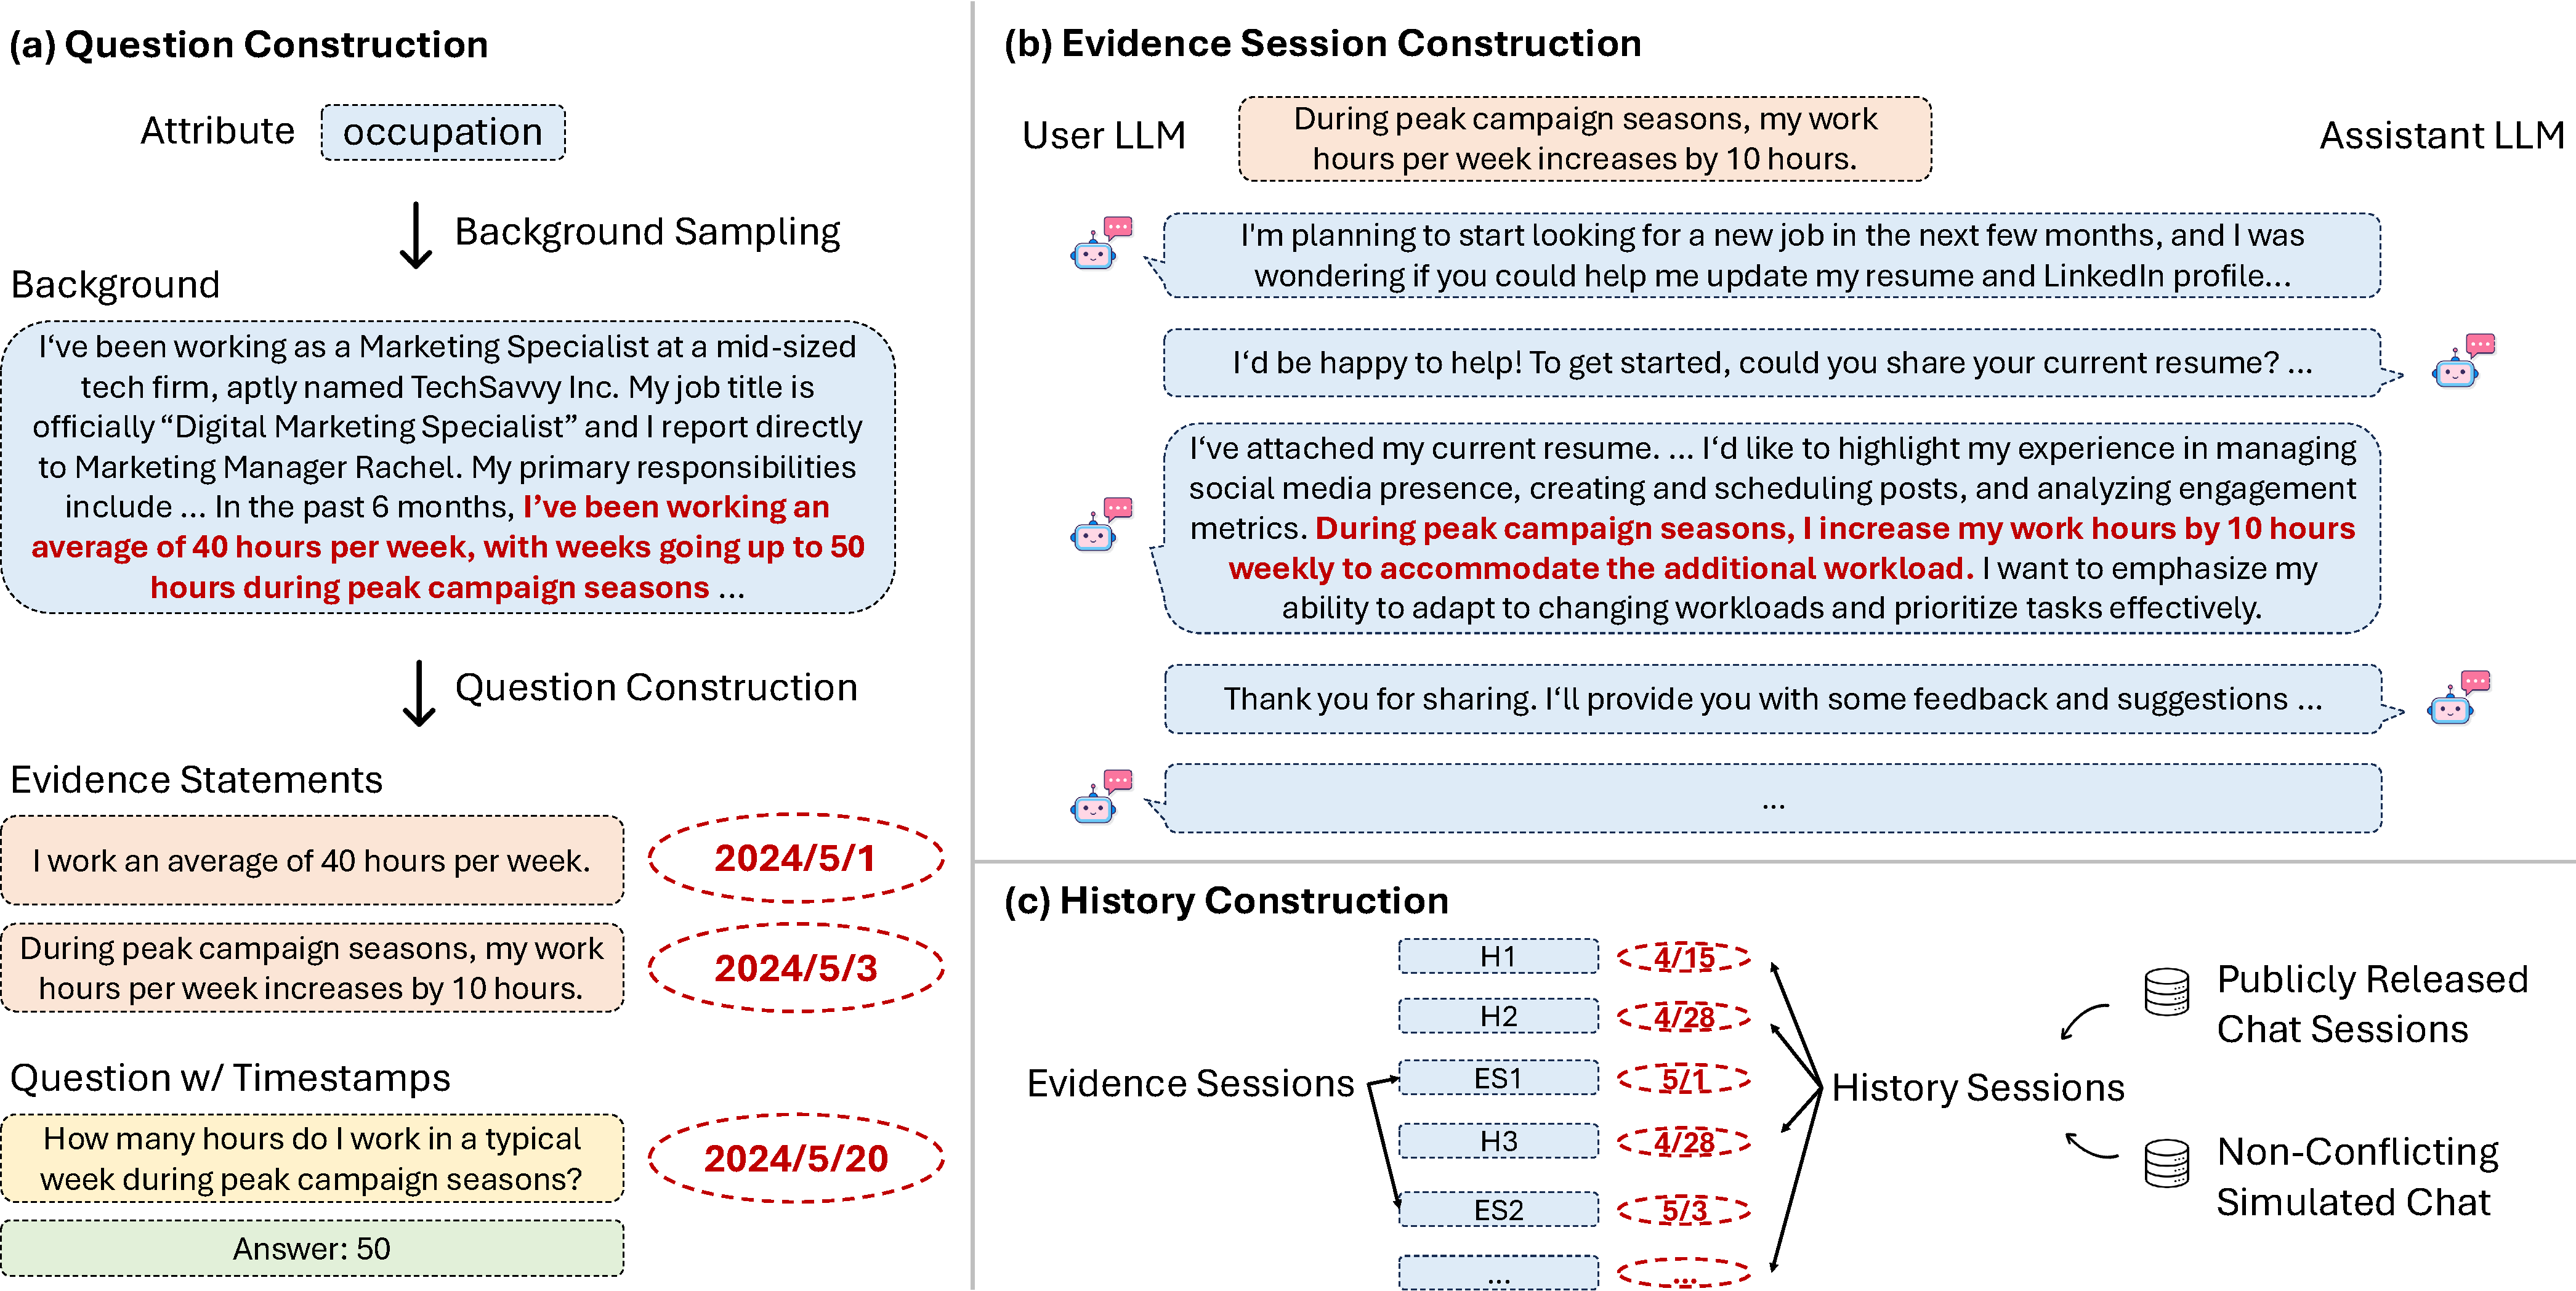
\includegraphics[width=0.98\textwidth]{figures/main_annotation_pipeline.pdf} 
 \vspace{-2mm}
  \caption{Data creation pipeline of \BENCHMARK{}. {(a) Human experts construct all the questions and evidence statements. (b) Then, the evidence sessions are LLM-simulated and human-edited. (c) The full user-AI chat history is constructed at test time, whose length is freely configurable.}}
 \label{fig:main-fig-benchmark-creation}
\vspace{-5mm}
\end{figure}

\paragraph{{History Compilation}} 

For each question, \BENCHMARK{} compiles a coherent user-AI chat history (\Cref{fig:main-fig-benchmark-creation}c). Our approach is analogous to the needle-in-a-haystack test \citep{kamradt2023needle}, which asks a model to retrieve brief information (the ``needle") embedded in a long document (the ``haystack"). In comparison, \BENCHMARK{} is more challenging and realistic as it involves retrieving and synthesizing information from multiple extended evidence sessions. Specifically, we sample a number of unrelated user-AI chat sessions, randomly insert the evidence sessions in the middle, and assign a plausible timestamp to all sessions. We draw the irrelevant sessions from two sources: (1) self-chat sessions simulated based on other non-conflicting attributes and (2) publicly released user-AI style chat data including ShareGPT \citep{zheng2023judging} and UltraChat \citep{ ding2023enhancing}. This design creates extensible realistic chat histories with minimal conflicts. While the pipeline allows us to compile chat histories of arbitrary length, we provide two standard settings: \BENCHMARK\textsubscript{\textsc{S}} ($\sim$115k tokens/question) and \BENCHMARK\textsubscript{\textsc{M}} (500 sessions, $\sim$1.5M tokens). 


\subsection{Evaluation Metric}

\paragraph{Question Answering} As the correct answers can take flexible forms, an exact matching strategy as in previous works can result in inaccurate evaluations. To address this, \BENCHMARK{} employs a LLM to assess response quality \citep{liu-etal-2023-g}. Specifically, we prompt-engineer  the \texttt{gpt-4o-2024-08-06} model via the OpenAI API. Our meta-evaluation study demonstrates that the evaluator achieves more than 97\% agreement with human experts. The prompts for each problem type as well as the human meta-evaluation details are presented in \Cref{appendix-evaluation–metric}.


\paragraph{Memory Recall} As \BENCHMARK{} contains human-annotated answer location labels, intermediate retrieval metrics can be easily calculated if the chat system exposes its retrieval results. We report Recall@$k$ and NDCG@$k$, where $k$ is the number of top items retrieved by the system.


\subsection{\BENCHMARK{} represents a significant challenge}
\label{section-benchmark-challenging}

Using \BENCHMARK, we conduct a pilot study on commercial systems and long-context LLMs.

\paragraph{Commercial systems} We evaluate two commercial systems that maintain a set of memorized user facts as the user chats with the assistant: ChatGPT \citep{openai_memory_2024} and Coze \citep{coze_memory_2024}. Since these systems only support memory features via their web interfaces, we randomly selected 97 questions and created a short chat history of 3-6 sessions (approximately 10x shorter than \BENCHMARK\textsubscript{\textsc{S}}). Human annotators interacted with the chat assistants session-by-session and turn-by-turn, and finally ask the question in a new session\footnote{All evaluations were conducted in the first two weeks of August 2024.}. In \Cref{fig:proof-of-difficulty-commercial-systems}, we compare this online memory evaluation with offline reading, where GPT-4o is prompted to answer with the complete history provided as context. Both ChatGPT and Coze exhibited significant performance drops compared to offline reading, underscoring the challenging nature of \BENCHMARK{}. We found ChatGPT tended to overwrite crucial information as the chat continues, while Coze often failed to record indirectly provided user information. We provide analyses in \Cref{appendix-manual-analysis}. Overall, this result highlights the \textbf{gap between building a seemingly personalized chat assistant by recalling isolated facts and demonstrating a genuinely strong memory ability}.


\begin{figure}[t]
 \vspace{-3mm}
 \centering
 \begin{subfigure}{0.49\textwidth}
 \centering
 \resizebox{0.9\linewidth}{!}{
 \begin{tabular}{c|c|c}
\toprule
\textbf{System}  & \textbf{LLM} & \textbf{Accuracy} \\ \midrule
Offline Reading & GPT-4o & 0.9184 \\
\midrule
\multirow{2}{*}{ChatGPT} & GPT-4o & 0.5773\\ 
 & GPT-4o-mini & 0.7113 \\ 
 \midrule
\multirow{2}{*}{Coze}& GPT-4o & 0.3299 \\ \
 & GPT-3.5-turbo & 0.2474 \\ 
 \bottomrule
\end{tabular}
}
\caption{Commercial memory-augmented chat assistants exhibit weak performance on \BENCHMARK. The accuracy of ChatGPT and Coze degrades by a large amount compared to directly reading the context (``Offline Reading") with the same LLM. Specifically, ChatGPT and Coze instantiated with GPT-4o exhibits 37\% and 64\% performance drop, respectively.}
 \label{fig:proof-of-difficulty-commercial-systems}
 \end{subfigure}
 \hfill
 \begin{subfigure}{0.49\textwidth}
 \centering
 \resizebox{0.9\linewidth}{!}{
\begin{tabular}{l c c c c}
\toprule
\textbf{Model} & \textbf{Size} & \textbf{Oracle} & \textbf{\textsc{S}} & \textbf{\% Drop} \\
\midrule
\rowcolor{gray!20} \multicolumn{5}{c}{\textbf{No Chain-of-Note}} \\
\midrule
GPT-4o & - & 0.870 & 0.606 & 30.3\%$\downarrow$ \\
Llama 3.1 Instruct & 70B & 0.744 & 0.334 & 55.1\%$\downarrow$ \\
Llama 3.1 Instruct & 8B & 0.710 & 0.454 & 36.1\%$\downarrow$ \\
Phi-3 128k Instruct & 14B & 0.702 & 0.380 & 45.9\%$\downarrow$ \\
Phi-3.5 Mini Instruct & 4B & 0.660 & 0.342 & 48.1\%$\downarrow$ \\
\midrule
% With CoT \\
\rowcolor{gray!20} \multicolumn{5}{c}{\textbf{With Chain-of-Note}} \\
\midrule
GPT-4o & - & 0.924 & 0.640 & 30.7\%$\downarrow$ \\
Llama 3.1 Instruct  & 70B & 0.848 & 0.286 & 66.3\%$\downarrow$ \\
Llama 3.1 Instruct & 8B & 0.710 & 0.420 & 40.8\%$\downarrow$ \\
Phi-3 128k Instruct & 14B & 0.722 & 0.344 & 52.4\%$\downarrow$ \\
Phi-3.5 Mini Instruct & 4B & 0.652 & 0.324 & 50.3\%$\downarrow$ \\
\bottomrule
\end{tabular}
}
 \caption{{Long-context LLMs exhibit large QA performance drops on \BENCHMARK\textsubscript{\textsc{S}} (column ``\textsc{S}"), compared to the accuracy of answering the questions based on only the evidence sessions (column ``Oracle").}}
 \label{fig:proof-of-difficulty-long-context}
 \end{subfigure}
 \caption{Pilot study of {(a)} commercial systems and {(b)} long-context LLMs on \BENCHMARK.}
 \label{fig:proof-of-difficulty}
 \vspace{-3mm}
\end{figure}

% \wenhao{We should (1) remove questions that are not in the final dataset and (2) compare with the long context setting}




\paragraph{Long-Context LLMs} While \BENCHMARK{} poses a significant challenge to online memory systems, is the benchmark easily tackled with offline reading over the entire history? In \Cref{fig:proof-of-difficulty-long-context}, we evaluated four advanced long-context LLMs on \BENCHMARK\textsubscript{\textsc{S}} (with a history length of approximately 115k tokens): GPT-4o, Llama 3.1 Instruct \citep{dubey2024llama}, and Phi-3 \citep{phi-3-technical-report}. Compared to the oracle retrieval setting (answering with only the evidence sessions as the context), these LLMs showed a 30\% to 60\% performance decline when tasked with reading the entire \BENCHMARK\textsubscript{\textsc{S}} history, regardless of whether the chain-of-note technique \citep{yu2023chain} was applied (discussed further in \Cref{section-design-choices}). As the histories in \BENCHMARK\textsubscript{\textsc{S}} is still short ($\sim$50 sessions), the performance is likely to further degrade as the interaction history expands. Overall, these findings suggest that \textbf{even the most capable current long-context LLMs struggle to manage an ever-growing interaction history without an effective memory mechanism}.

